%----------------------------------------------------------
% Main format settings
%----------------------------------------------------------
\documentclass{article}
\usepackage{graphicx}
\usepackage{authblk}
\setlength{\textwidth}{16cm}
\setlength{\oddsidemargin}{0pt}
\setlength{\evensidemargin}{0pt}
\setlength{\topmargin}{0cm}
\usepackage{caption} 
\captionsetup[table]{skip=10pt}
\usepackage{mathtools}
\usepackage{graphicx}
\usepackage{hyperref}
\usepackage[utf8]{inputenc}
 
\usepackage{listings}
\usepackage{float}
\usepackage{xcolor}
\usepackage{subfig}
\definecolor{codegreen}{rgb}{0,0.6,0}
\definecolor{codegray}{rgb}{0.5,0.5,0.5}
\definecolor{codepurple}{rgb}{0.58,0,0.82}
\definecolor{backcolour}{rgb}{0.95,0.95,0.95}
 
\lstdefinestyle{mystyle}{
    backgroundcolor=\color{backcolour},   
    commentstyle=\color{codegreen},
    keywordstyle=\color{magenta},
    numberstyle=\tiny\color{codegray},
    stringstyle=\color{codepurple},
    basicstyle=\ttfamily\footnotesize,
    breakatwhitespace=false,         
    breaklines=true,                 
    captionpos=b,                    
    keepspaces=true,                 
    numbers=left,                    
    numbersep=5pt,                  
    showspaces=false,                
    showstringspaces=false,
    showtabs=false,                  
    tabsize=2
}
\lstset{style=mystyle}
%----------------------------------------------------------
% Start of the document
%----------------------------------------------------------
\begin{document}
%----------------------------------------------------------
% Title and authors sections
%----------------------------------------------------------
\title{Restricted Three-Body Problem: Determining the Motion of Three Gravitating Bodies}
\author{Bernardo A. Roque Carri\'{o}n, Jomarie Jim\'{e}nez Gonz\'{a}lez, 

Jordan A Caraballo-Vega, Pablo Negr\'{o}n Marrero}
\affil{Department of Mathematics, UPR-Humacao}
\maketitle % this produces the title block
%----------------------------------------------------------
% Introduction
%----------------------------------------------------------
\section{Introduction}

The three-body problem has been around for more than 300 years \cite{Musielak}. It was formulated and studied by Newton in his Principia, and subject of many investigations by the best minds of the 18th and 19th centuries \cite{Frank}. The problem initially considered by Newton was the motion of the Earth and the Moon around the Sun, taking into account future and past motions of the bodies to be uniquely determined based solely on their present positions and velocities \cite{Frank}. Newton solved the two-body problem for the orbit of the Moon around the Earth; but only considered the effects of the Sun on this motion \cite{Musielak}. In recent decades, this problem has been reformulated to study the dependency of star clusters and the nuclei of active galaxies on the interactions between black hole binaries and additional systems. 

The general three-body problem remains unsolved today. Historical simplifications to this problem have enabled the determination of finite solutions for the orbits of these complex systems using modern computational hardware and methods. The first and simplest solution to the three-body problem was found by Euler in 1967, followed by Lagrange in 1772. The basis for the modern theory of the restricted three-body problem was developed by Jacobi, Delaunay, and Hill \cite{Frank}. Some simplifications can be made when dealing with the three-body problem in Sun-planet-asteroid systems since the mass of the asteroid is always negligible when compared to the mass of the Sun or a planet. Taking into account these conditions, the gravitational influence of the asteroid on the planet and the Sun can be omitted from the theory.

In this work, we study the plannar circular restricted three-body problem where the first two bodies move in circular orbits around their joint centre-of-mass and the motion of the third body is confined to the plane of the circles. For this work, the centre-of-mass is taken as the origin and the plane of the circles is taken as the x-y-plane. A set of scripts were developed to study the orbits of these systems in presence of velocity and position changes. At the end, a set of possible sources of errors are described and analyzed for the future improvement of this method.

\section{Materials and Methods}

This section describes the processes and techniques used to model and solve the restricted three-body problem for specified conditions. The cases studied in this manuscript have been taken from the University of Cambridge Restricted Three-Body Problem lecture provided by professor P. Negr\'{o}n as a requirement for the Numerical Analysis class. This project prioritizes the use of numerical methods for the analysis of the restricted three-body problem.
 
\subsection{Software}

The models and simulations developed for this work were generated using Octave. The function ode45, a black-box ODE solver, was used to find numerical solutions of the proposed differential equations systems. This specific function was selected due to its ability to automatically adapt the time-step according to specified absolute and relative error tolerances. 

\subsection{Hardware}

An AlienWare 17 Intel Core i7 CPU at 2.80GHz × 8 with GeForce GTX 1060 and 16GB of memory with Ubuntu 18.04.03 LTS was used for this work. Simulations developed for this project have proven to be resource intensive, but non-invasive in memory performance. After five consecutive simulations, the average execution time is approximately 62 seconds, with less than 1GB of memory required for the Octave process (Table 1). Thus, the computing time and memory recorded indicates that it is feasible tu run the proposed simulations in commodity based hardware. More complex systems will require high performance computing solutions.

\begin{table}[h!]
  \begin{center}
    \caption{Average system performance during simulation execution time of the Octave process.}
    \label{tab:table1}
    \begin{tabular}{c|c|c|c} 
      \textbf{Run} & \textbf{\% CPU} & \textbf{Memory (MiB)} & \textbf{Execution Time (s)}\\
      \hline
      1 & 12 & 65.8 & 61.05\\
      2 & 12 & 62.9 & 60.27\\
      3 & 12 & 64.7 & 61.96\\
      4 & 12 & 64.0 & 62.74\\
      5 & 12 & 67.9 & 61.78\\
      \hline
      Average & 12 & 65.1 & 61.56\\
      \hline
    \end{tabular}
  \end{center}
\end{table}

\subsection{General Restricted Three-Body Problem}

Several modifications need to be addressed in order to transform the general three-body problem into a restricted system. The first step is to represent the first two bodies as stationary. Scalings are chosen so that the angular velocity and the distance between the two bodies is 1. Therefore, the only parameter appearing in this restricted system is the mass ($\mu$) where $\mu$ $\in$ (0, 0.5] such that the two masses are in the ratio $\mu$ : 1 - $\mu$ and are situated at the points ($\mu$ - 1, 0) and ($\mu$, 0) respectively. These systems will now on be referred as \textit{Pl} and \textit{Ph}.

\newpage

Then, the equation of motion of the third body, whose position at time \textit{t} is given by (\textit{x}(\textit{t}),\textit{y}(\textit{t})), can be written as:

\begin{equation}\label{1a}
\ddot{x} - 2\dot{y} = - \frac{\partial \Omega}{\partial x},
\end{equation}

\begin{equation}\label{1b}
\ddot{y} + 2\dot{x} = - \frac{\partial \Omega}{\partial y},
\end{equation}

where $\Omega$ is the potential of the centrifugal and gravitational forces given by:

\begin{equation}\label{2}
\Omega = - \frac{1}{2} (x^2 + y^2) - \frac{\mu}{\sqrt{(x+1-\mu)^2+y^2}} - \frac{1 - \mu}{\sqrt{(x-\mu)^2+y^2}}
\end{equation}

Despite this substantial restriction to the three-body problem, it is not possible to solve the system (\ref{1a}), (\ref{1b}), and (\ref{2}) analytically. Thus we proceed to convert it to an order one system and approximate its numerical solutions using Octave and additional numerical methods.

\subsection{J Constant Following Motion}

The purpose of this section is to show from (\ref{1a}) and (\ref{1b}) that the quantity:

\begin{equation}\label{J}
J = \frac{1}{2} (\dot{x}^2 + \dot{y}^2) + \Omega(x,y)
\end{equation}

is constant following the motion. For this problem, the fact that J is constant provides not only a useful constraint
on the behaviour of solutions, but also another possible check on numerical accuracy. Observe that by applying the derivative in respect to time to this system we obtain:

\begin{equation}\label{Jprove}
        \begin{split}
            \frac{dJ}{dt} & = \frac{1}{2} (2\dot{x} x^2 + 2\dot{y}y^2) + \frac{d\Omega(x,y)}{dt} \\
           & = \dot{x} (2\dot{y} - \frac{d\Omega}{dx}) + \dot{y}(-2\dot{x} - \frac{d\Omega}{dy}) + \frac{d\Omega}{dx}\dot{x} + \frac{d\Omega}{dy}\dot{y} \\ 
           \frac{dJ}{dt} & = 0 \\                 
        \end{split}
\end{equation}

As shown in (\ref{Jprove}), all of the terms can be cancelled after applying the derivative. Thus we can conclude J is constant following the motion. Since the first term from (\ref{J}) refers to the kinetic energy and the second term refers to the potential energy, we can deduce that trajectories must be confined to the region by:

\begin{equation}\label{energy}
\Omega(x,y) \leq \frac{1}{2} (\dot{x}^2 + \dot{y}^2) + \Omega(x,y) = \frac{1}{2} (u_0^2 + v_0^2) + \Omega(x_0,y_0)
\end{equation}

where $x_0$, $y_0$, $u_0$ and $v_0$ are the initial values of x, y, $\dot{x}$ and $\dot{y}$ respectively. Thus we can conclude that:

\begin{equation}\label{energyconc}
\Omega(x,y) \leq \frac{1}{2} (u_0^2 + v_0^2) + \Omega(x_0,y_0)
\end{equation}

By determining this external forbidden region we can make sure that orbit trajectories are being calculated properly. This in order to avoid error propagation coming from the ODE solver or the introduction of unsuitable initial parameters to the system. Figure 1 shows an orbit (purple) and a not-to-scale forbidden region (red) surrounding the trajectories of this orbit. By knowing that J is constant and the forbidden region can be calculated, we proceed to write a program to solve numerically the system (\ref{1a}), (\ref{1b}), and (\ref{2}) given suitable initial conditions on x, y, $\dot{x}$ and $\dot{y}$.

\begin{center}
  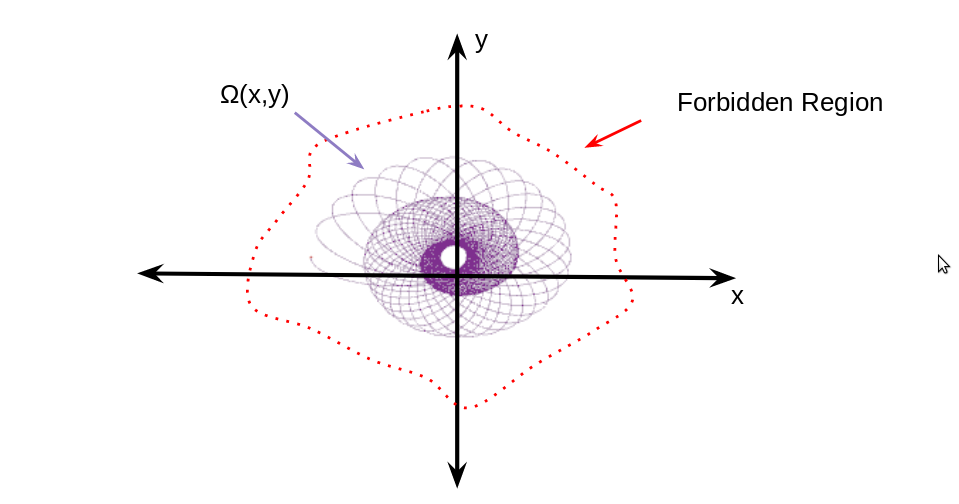
\includegraphics[width=0.5\linewidth]{confinedarea}
\end{center}

\begin{center}
   \textit{Figure 1. Not-to-scale representation of the confined region (red) that encompases the boundaries for the trajectories of the selected orbit (purple). The forbidden region is given by (\ref{energyconc}).}
\end{center}

The first step before developing this program is to transform the equations into an order one system. Therefore, we take:

\begin{equation}\label{transform1}
        \begin{cases}
            \ddot{x} - 2 \dot{y} & = - \frac{d \Omega}{dx} \\
            \ddot{y} + 2 \dot{x} & = - \frac{d \Omega}{dy} \\                
        \end{cases}
\end{equation}

and transform them using:

\begin{equation}\label{transform2}
   \begin{cases}
    u_1(t) = x(t) \\
    u_2(t) = \dot{x}(t) \\
    u_3(t) = y(t) \\
    u_4(t) = \dot{y}(t) \\
  \end{cases}     
\end{equation}

Thus we get the following order one system:

\begin{equation}\label{transform3}
   \begin{cases}
    \dot{u}_1(t) = u_2(t) \\
    \dot{u}_2(t) = 2 u_4(t) - \frac{d \Omega}{dx} (u_1(t),u_3(t)) \\
    \dot{u}_3(t) = u_4(t) \\
    \dot{u}_4(t) = - 2 u_2(t) - \frac{d \Omega}{dy} (u_1(t),u_3(t)) \\
  \end{cases}     
\end{equation}

Note that we end up with a four equation system where $\dot{x}$ and $\dot{y}$ represent initial velocities, and x and y represent initial positions. The transformation done to this system is needed to simplify the solutions to be calculated by the Octave program.

\newpage

These equations are then added to an Octave function as follows:
 
\lstinputlisting[language=Octave]{prob3b.m}

Then, we proceed to use this function by adding the appropiate initial parameters to the ODE solver in an additional script. Finally, trajectories calculated by the ODE45 solver are plotted and visualized with the following program:

\lstinputlisting[language=Octave]{simulationorig.m}

It is imperative to define ODE Absolute Tolerance and Max Step options when using Octave ODE solver. If these parameters are not specified, the numerical solutions given by the system will not appear to be smooth at the time of being visualized (this will be addressed in section 3.4).

\subsection{Copenhagen Problem}

To analyze the Copenhagen problem we assume that the third body is a spacecraft, with the first two heavy bodies being co-orbiting planets of equal mass. Additionally, we assume that the spacecraft is extremely close to \textit{Ph} so that the gravitational attraction from \textit{Pl} can be discarded. Thus we can also discard the centrifugal force term. Figure 2 includes a visual representation of this system. Now, lets assume $\mu$ = 0.5, then equation (\ref{2}) may be approximated by:

\begin{equation}\label{copen}
\Omega = - \frac{0.5}{ \sqrt{ (x - 0.5)^2+ y^2}}
\end{equation}

Question 2 from the University of Cambridge lecture requires us to show that in polar co-ordinates with:

\begin{equation}\label{polar}
x(t) - \mu = r(t) cos \theta(t), y(t) = r(t) sin \theta(t)
\end{equation}

\newpage

the approximate system (\ref{1a})–(\ref{1b}) with (\ref{copen}) is equivalent to

\begin{equation}\label{polara}
\dot{\theta} = -1 + kr^{-2}, \ddot{r} = -V'(r)
\end{equation}

where \textit{k} is an arbitrary constant and \textit{V'(r)} is to be found, and has analytic solutions  for particular initial conditions with the spacecraft in a circular orbit of radius \textit{a} about \textit{Ph}, where \textit{a} can take any value. Therefore we start with the following system:

\begin{equation}\label{copenstart}
   \begin{cases}
      \ddot{x} - 2 \dot{y} & = - \frac{d \Omega}{dx} = - \frac{0.5 (x-0.5)}{ ((x - 0.5)^2+ y^2)^{\frac{3}{2}}}\\
      \ddot{y} + 2 \dot{x} & = - \frac{d \Omega}{dy} = - \frac{0.5 y}{ ((x - 0.5)^2+ y^2)^{\frac{3}{2}}}\\                
   \end{cases}   
\end{equation}

Then, taking the parameters given by (\ref{polar}), we end up with the following systems:

\begin{equation}\label{copensecond}
   \begin{cases}
      \dot{x} = \dot{r} cos\theta - r\dot{\theta} sin\theta \\
      \dot{y} = \dot{r} sin\theta + r\dot{\theta} cos\theta \\
   \end{cases}   
\end{equation}


\begin{equation}\label{copenthird}
\begin{cases}
\ddot{x} = \ddot{r} cos\theta - 2\dot{r}\dot{\theta} sin\theta - r(\dot{\theta})^2 cos \theta - r\ddot{\theta} sin \theta\\
\ddot{y} = \ddot{r} sin\theta + 2\dot{r}\dot{\theta} cos\theta - r(\dot{\theta})^2 sin \theta + r\ddot{\theta} cos \theta\\
\end{cases}   
\end{equation}

Therefore, using (\ref{copenstart}), (\ref{copensecond}) and (\ref{copenthird}) we obtain:

\begin{equation}\label{copen3}
\begin{cases}
\ddot{r} cos\theta - 2\dot{r}\dot{\theta} sin\theta - r(\dot{\theta})^2 cos \theta - r\ddot{\theta} sin \theta - 2\dot{r}sin\theta - 2r\dot{\theta} cos \theta = - \frac{0.5cos\theta}{r^2}\\
\ddot{r} sin\theta + 2\dot{r}\dot{\theta} cos\theta - r(\dot{\theta})^2 sin \theta + r\ddot{\theta} cos \theta + 2\dot{r}cos\theta - 2r\dot{\theta} sin\theta = - \frac{0.5sin\theta}{r^2}\\
\end{cases}   
\end{equation}

Then, taking:

\begin{equation}\label{copenfourth}
        \begin{split}
            (cos\theta)e_1 & + (sen\theta)e_2, and  \\
            (sin\theta)e_1 & - (cos\theta)e_2 \\
        \end{split}
\end{equation}

we end up with:

\begin{equation}\label{copen5}
\begin{cases}
\ddot{r}-r(\dot{\theta})^2 -2r\dot{\theta} =-\frac{0.5}{r^2}\\
-2\dot{\theta}\dot{r}-r\ddot{\theta} -2\dot{r} =0\\
\end{cases}   
\end{equation}

By solving for $\dot{\theta}$ from (\ref{copen5}) we get:

\begin{equation}\label{copen6}
\begin{split}
\ddot{\theta} & = \frac{-2\dot{r}}{r} (1+\dot{\theta})\\
\frac{\ddot{\theta}}{(1+\dot{\theta})} &=\frac{-2\dot{r}}{r}\\
\end{split}
\end{equation}

\newpage

Note that (\ref{copen6}) has the form of $\int \frac{du}{u} = ln(u)$. Therefore:

\begin{equation}\label{copen7}
\begin{split}
\int \frac{\ddot{\theta}}{(1+\dot{\theta})} &= \int \frac{-2\dot{r}}{r} + c\\
ln (1+\dot{\theta}) &= ln(r^{-2}) + c \\
e^{lnr^{-2}+c} &= e^c r^{-2} \\
1+\dot{\theta} &= kr^{-2} \\
\end{split}
\end{equation}

Thus:

\begin{equation}\label{copen8}
\dot{\theta} = -1 + kr^{-2}
\end{equation}

Now, solving for $\ddot{r}$ from (\ref{copen5}) and with the value of $\dot{\theta}$ calculated above we get:

\begin{equation}\label{copen9}
\ddot{r} = -r + \frac{k^2}{r^{3}} - \frac{0.5}{r^2}
\end{equation}

which can be rewritten as:

\begin{equation}\label{copen10}
\ddot{r} = -V'(r)
\end{equation}

Thus we can conclude that:

\begin{equation}\label{copen10}
\begin{cases}
\dot{\theta} = -1 + kr^{-2} \\
\ddot{r} = -V'(r) \\
\end{cases}
\end{equation}

Note that the constant \textit{k} is related to \textit{a} by:

\begin{equation}\label{copen10}
\begin{cases}
k & = 1 + a^2\dot{\theta} \\
k & = \sqrt {a^4 + 0.5a }\\
\end{cases}
\end{equation}

Therefore, since \textit{a} must be positive, we can conclude that as \textit{a} increases, \textit{k} increases. Which means that \textit{k} is proportional to the size of \textit{a}.

\begin{center}
  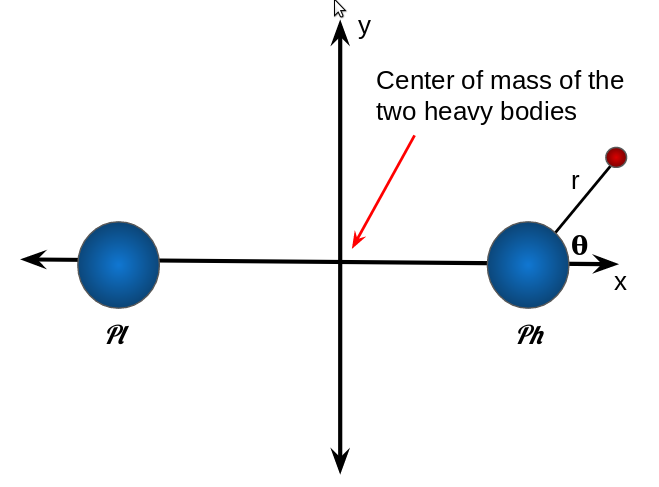
\includegraphics[width=7cm,height=4.5cm]{copenhagendiagram}
\end{center}

\begin{center}
   \textit{Figure 2. Representation of the Copenhagen problem. The spacecraft is close enough to \textit{Ph} so that \textit{Pl} gravitational forces can be discarded. The angle between the spacecraft (red) and \textit{Ph} is given by $\theta$.}
\end{center}

Given these solutions, we can proceed to adjust our Octave program to solve (\ref{1a})-(\ref{1b}) with $\Omega$ specified by (\ref{copen}). Note that the new adaptation for the Copenhagen problem is given by:

\lstinputlisting[language=Octave]{copenh.m}

Then, a script with an extremely low Absolute and Relative tolerance was developed to run the simulation of this system given specific parameters. Different values of \textit{a} were tested in order to reproduce the analytic circular-orbit solutions. The following program was given by professor P. Negr\'{o}n:

\lstinputlisting[language=Octave]{copenh_driver.m}

\subsection{Closer Look to the Forbidden Region}

Question 3 from the University of Cambridge lecture proposes a more in detail analysis to the change in the forbidden area by considering the original system given by (\ref{1a}), (\ref{1b}), and (\ref{2}) with additional changes in the initial conditions. Therefore, we take: \textit{x = 0.32}, \textit{y = 0}, \textit{$\dot{x}$ = 0}, \textit{$\dot{y}$ = $v_0$} with \textit{$v_0$} = -1.0, -1.5, -1.73, -1.78, -1.853, -1.858, -2.3 and -2.31 in turn and integrate the system from \textit{t = 0} to \textit{t = 30}. Then, an Octave program was developed to display the trajectory in the (x,y) plane, and the forbidden region $\Omega(x,y) > J$ on the same plot using the contour technique:

\lstinputlisting[language=Octave]{question3contor.m}

An assessment of the accuracy of the values of x and y at t = 30 is done in section 3.4.

\section{Results and Analysis}

This section includes results found by running the proposed simulations of the general restricted three-body problem and the Copenhagen problem. Numerical approximations of the trajectories for each system were calculated using Octave software. Additional details have been included below.

\subsection{General Restricted Three-Body Problem}

An Octave program was developed to visualize several systems by varying the initial parameters given to find the trajectories of the smallest system. Figure 3 represents a change in the initial position of the smallest body in the system. It was observed that small variations to this position affect drastically the trajectory of the orbit. 

\begin{center}
  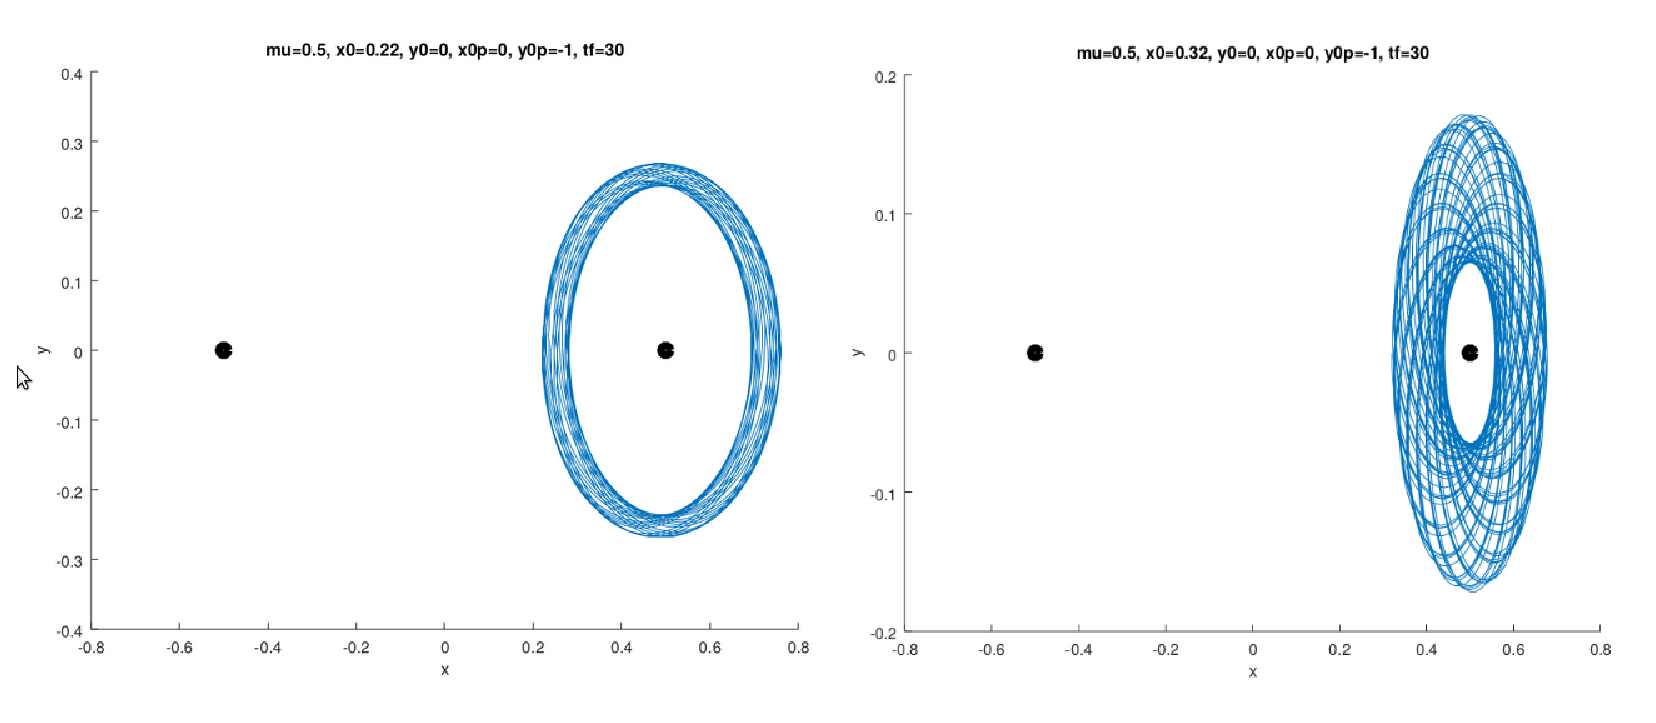
\includegraphics[width=16cm,height=5.5cm]{question1_022_032.eps}
\end{center}

\begin{center}
   \textit{Figure 3. Simulations with initial velocity of -1.0 and tf=30. (left) Trajectory of a system with initial position parameter at 0.22. (right) Trajectory of a system with initial position parameter at 0.32. }
\end{center}

Figure 4 shows two additional simulations when varying the initial velocity of the system. Note that small changes in the initial velocity of the system produces a big change in the trajectory. An increase in the velocity produced a wider orbit, which means that a larger distance was traveled.

\begin{center}
  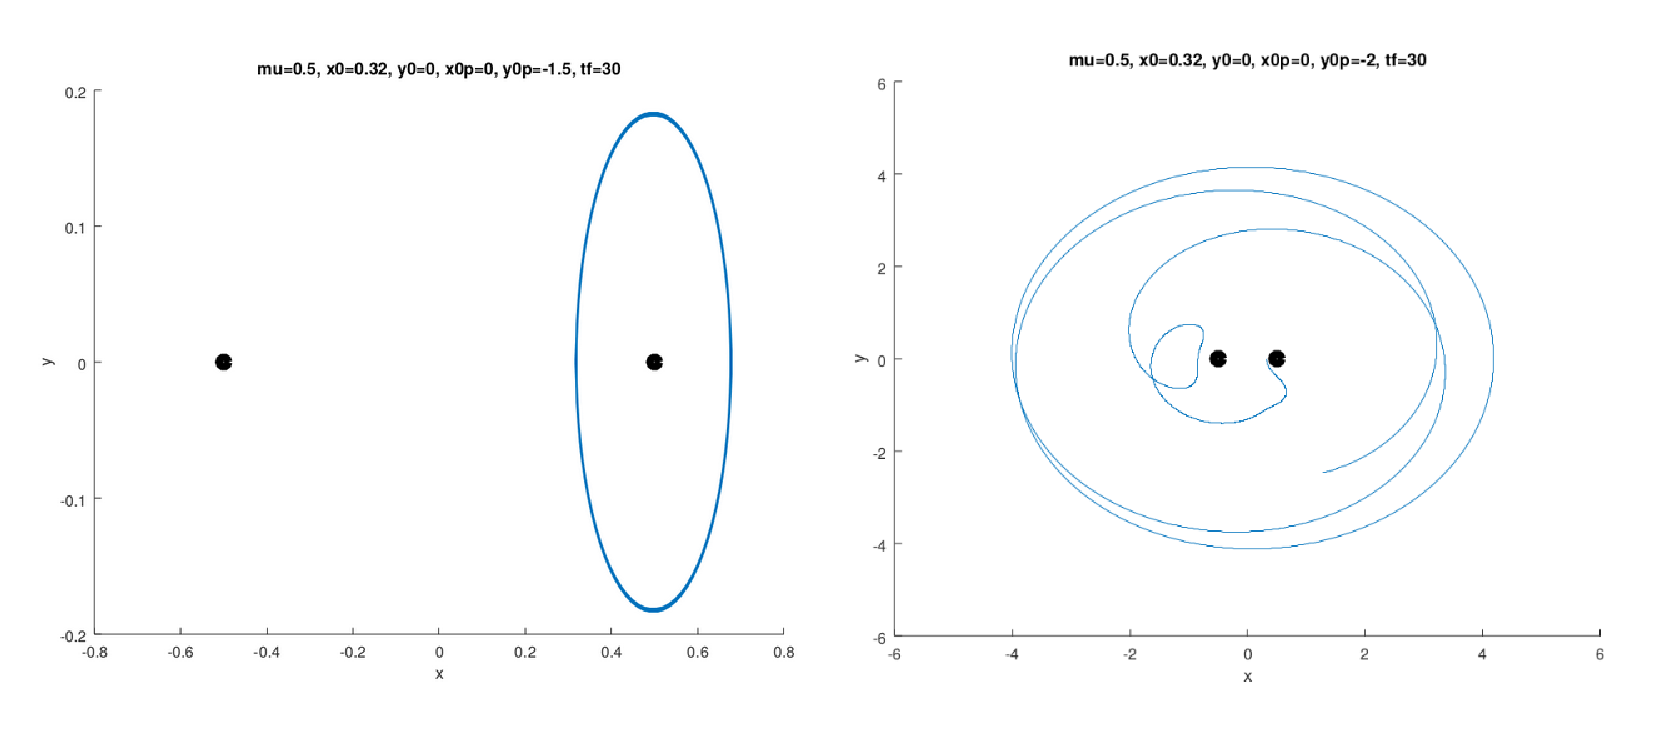
\includegraphics[width=16cm,height=5cm]{question1_vel.eps}
\end{center}

\begin{center}
   \textit{Figure 4. Simulations with initial position of 0.32 and tf=30. (left) Trajectory of a system with initial velocity parameter at -1.5. (right) Trajectory of a system with initial velocity parameter at -2.0. }
\end{center}

Thus we can conclude that both position and velocity initial parameters affect drastically the trajectory of the smallest system.

\subsection{Copenhagen Problem}

Several simulations were executed to analyze the effect of additional initial parameters in the Copenhagen problem where the centrifugal force from the furthest heavy body is discarded. Figure 5 shows two simulations where the initial positions are varied, and Figure 6 shows two simulations where the velocity parameter is varied.

\begin{center}
  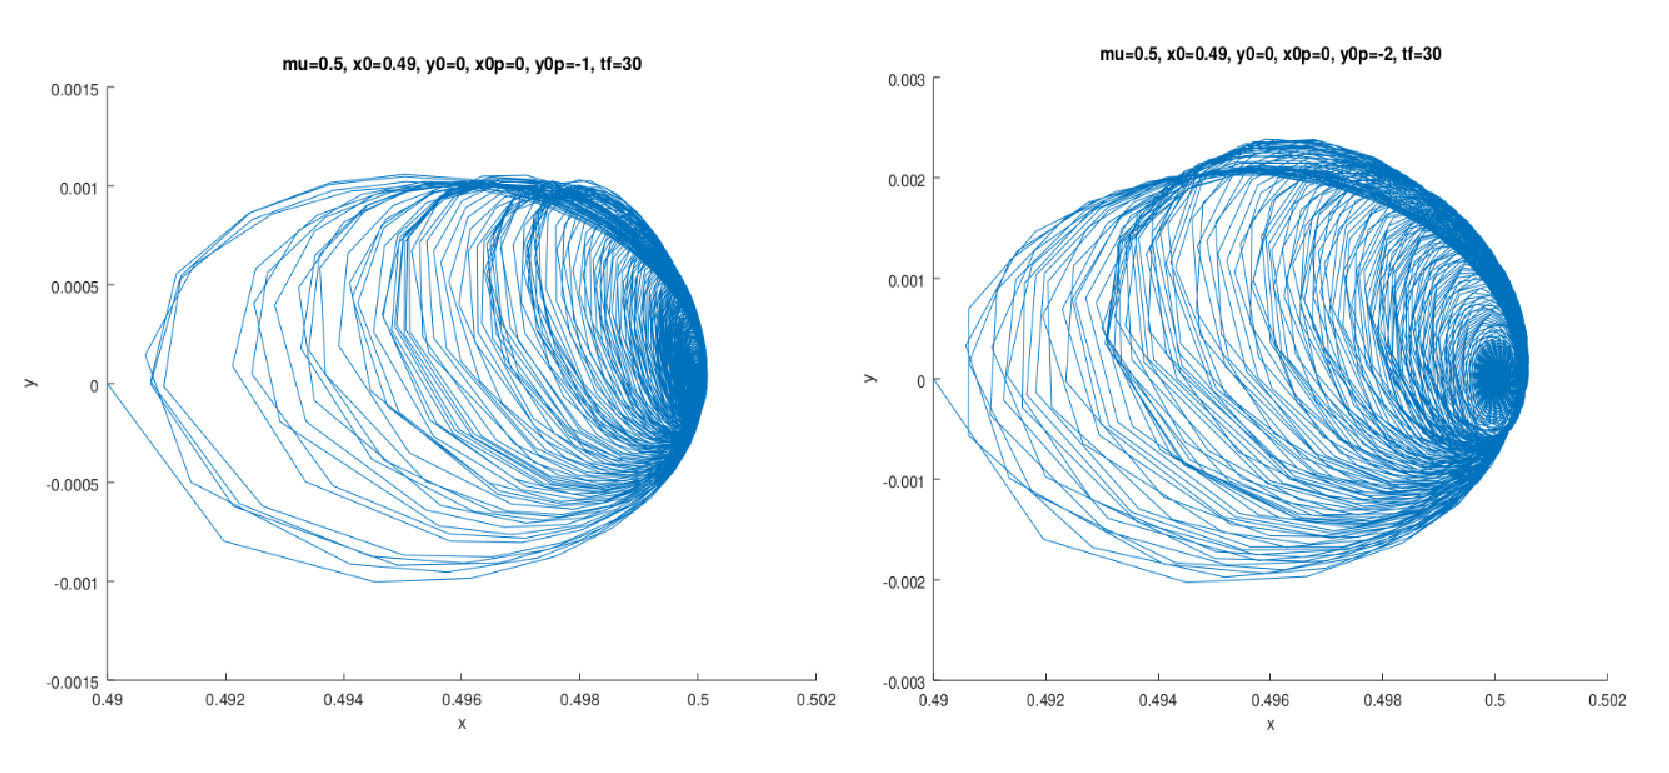
\includegraphics[width=16cm,height=5cm]{question2_vel.eps}
\end{center}

\begin{center}
   \textit{Figure 5. (left) Trajectory of a system with initial velocity parameter -1.0. (right) Trajectory of a system with initial velocity parameter -2.0.}
\end{center}

\begin{center}
  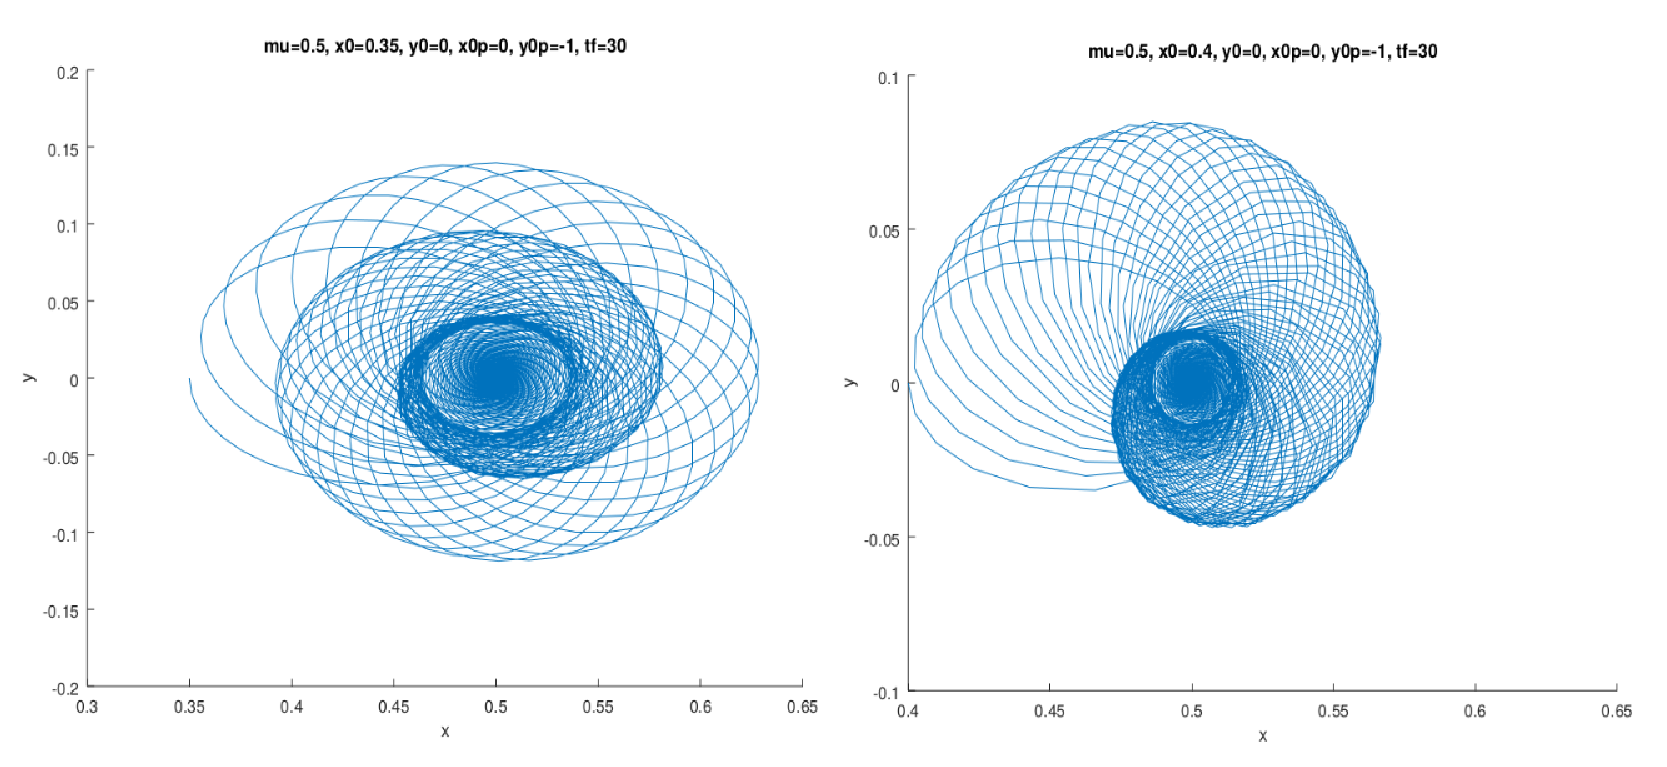
\includegraphics[width=16cm,height=5cm]{question2_pos.eps}
\end{center}

\begin{center}
   \textit{Figure 6. (left) Trajectory of a system with initial position parameter at 0.35. (right) Trajectory of a system with initial position parameter at 0.40.}
\end{center}

As shown, there are small variations in the trajectory when the velocity parameter is increased in the Copenhagen problem. On the other hand, small changes to the position of the third body drastically affect its trajectory. By adding the parameters for \textit{k} and by fixing \textit{$x_0$ = 0.49} we get \textit{a = |$x_0$-mu| = 0.49-0.50 = 0.01}, thus we were able to accurately reproduce the analytic circular-orbit solutions for the Copenhagen problem (Figure 7) with \textit{a = 0.01}.

\begin{center}
  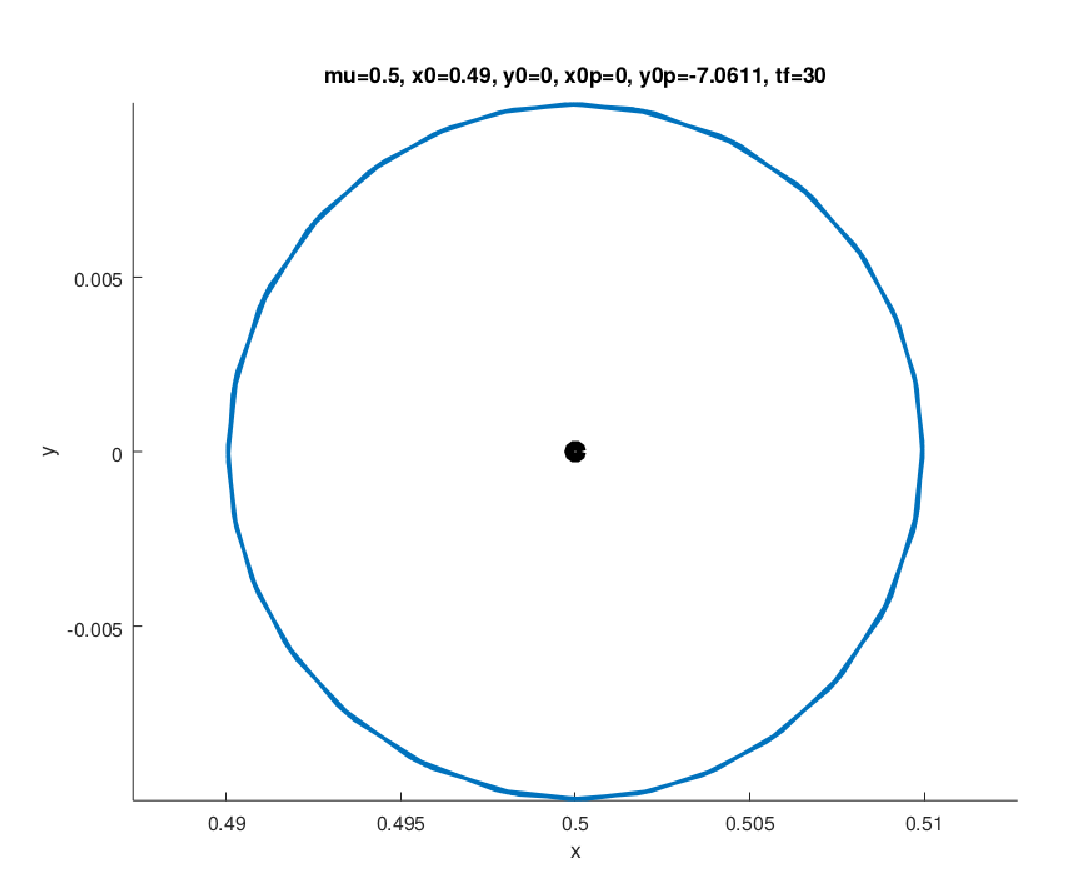
\includegraphics[width=10cm,height=7.5cm]{circularorbit.eps}
\end{center}

\begin{center}
   \textit{Figure 7. Analytic circular-orbit of the Copenhagen problem. The black spot in the center of the figure represents the heavy body closest to the smallest body. The furthest body was ommitted in this representation since the forces coming from this body are discarded by the definition of the Copenhagen problem.}
\end{center}

\subsection{Closer Look to the Forbidden Region}

Question 3 from the University of Cambridge lecture requires us to visualize the forbidden region of the trajectories of the smallest system at different velocities using (\ref{1a}), (\ref{1b}), and (\ref{2}). The following figures include the trajectories and forbidden region for each initial velocity.

\begin{center}
  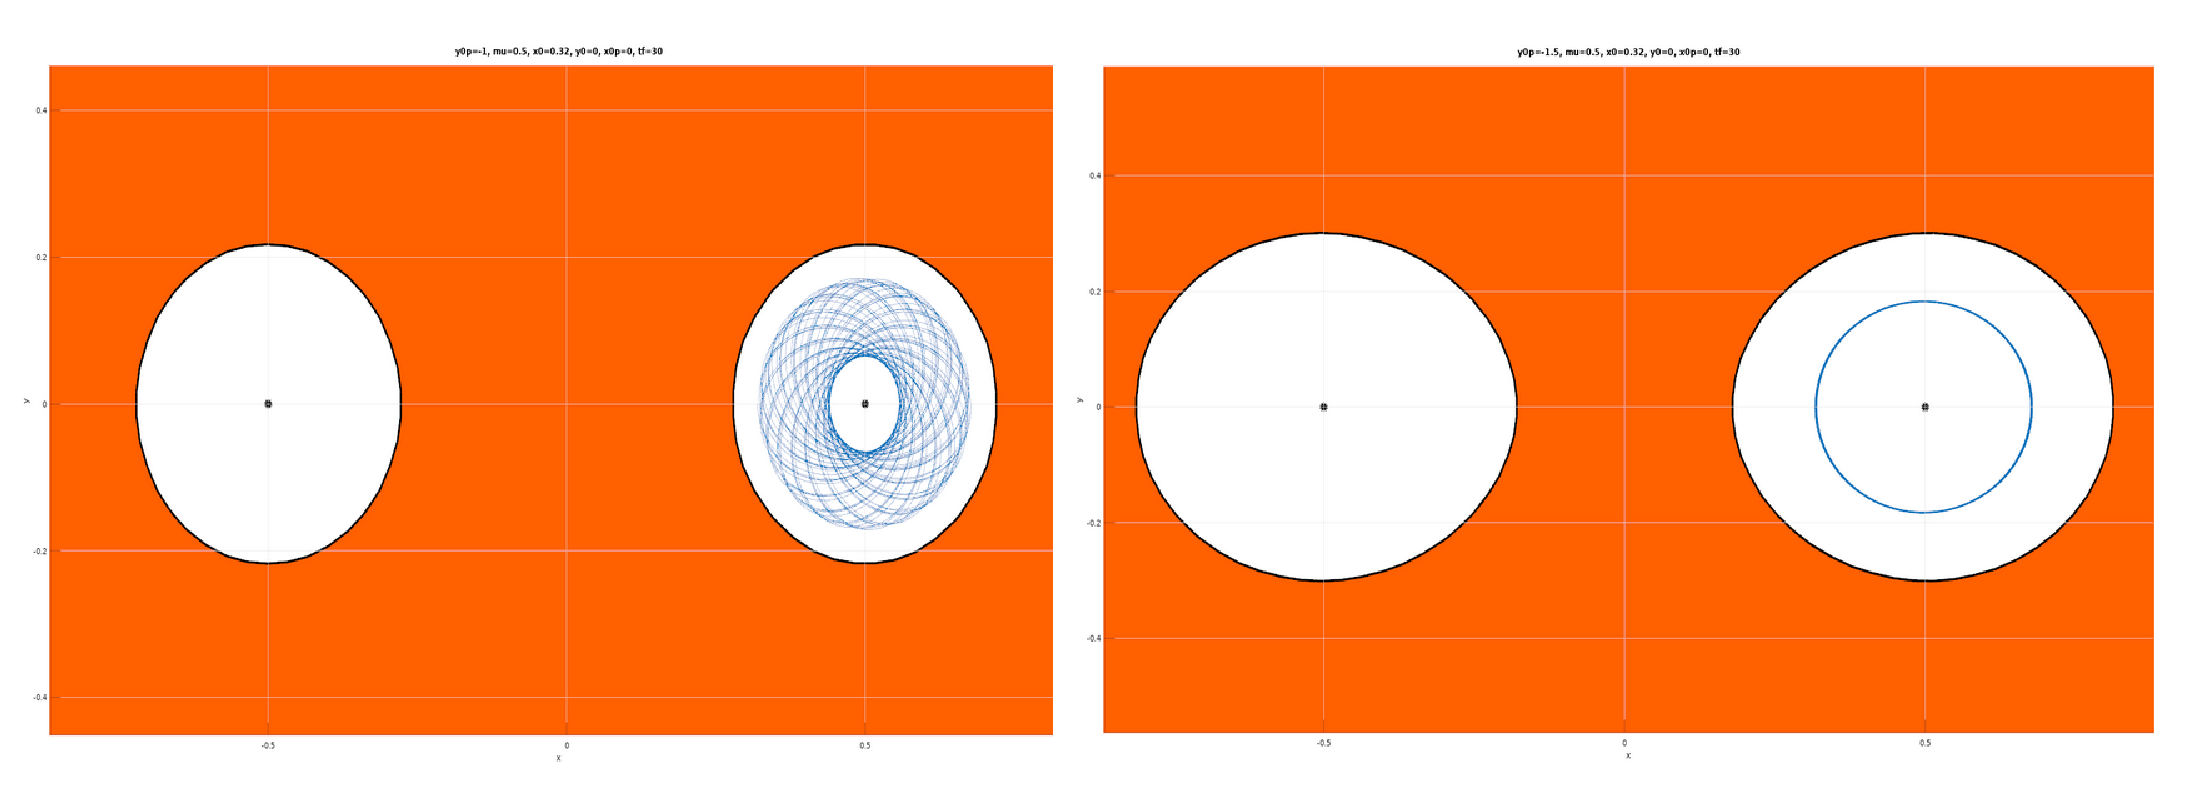
\includegraphics[width=16cm,height=5.5cm]{cont-first.eps}
\end{center}
\begin{center}
  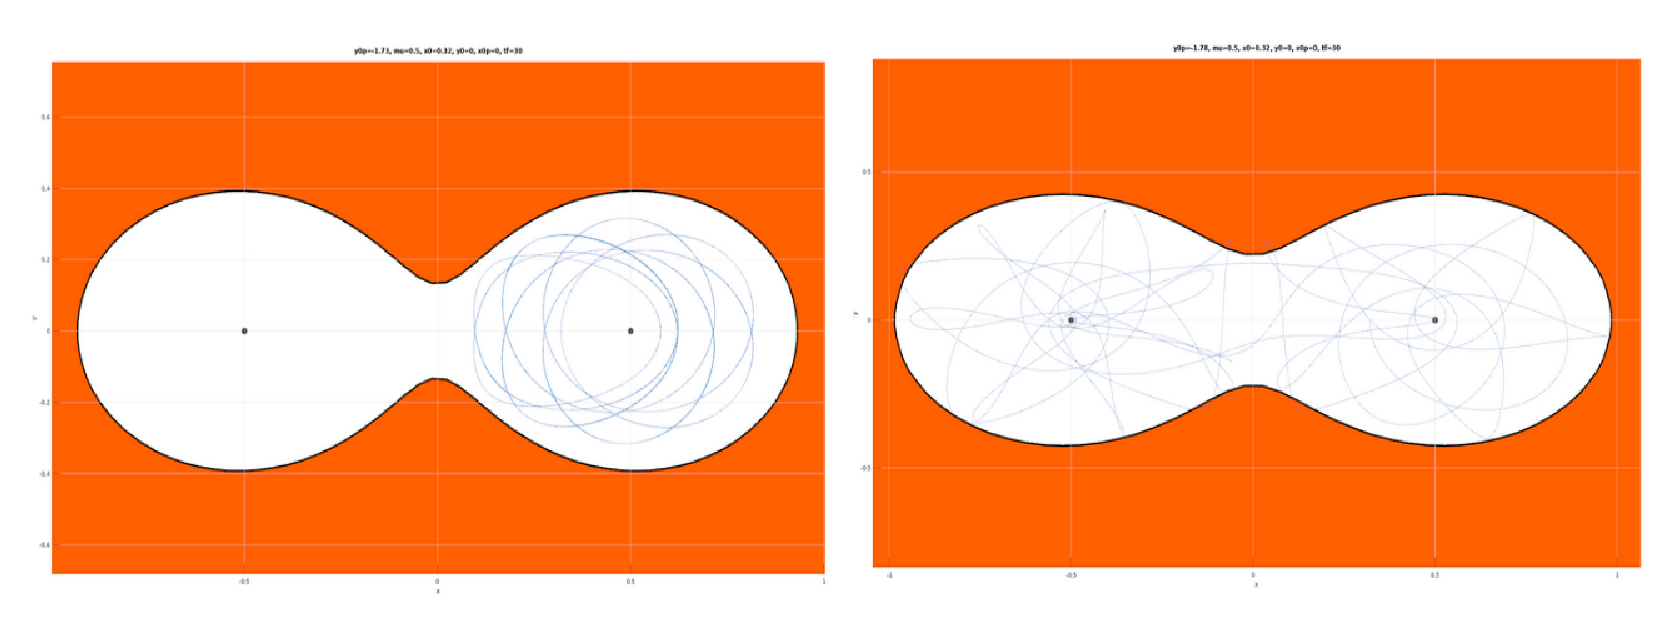
\includegraphics[width=16cm,height=5.5cm]{cont-second.eps}
\end{center}

\begin{center}
   \textit{Figure 8. Countour plots of the trajectories and the forbidden region. (upper left) Trajectory of a system with initial velocity parameter -1.0. (upper right) Trajectory of a system with initial velocity parameter -1.5. (lower left) Trajectory of a system with initial velocity parameter -1.73, and (lower right) shows the trajectory of a system with initial velocity parameter -1.78.}
\end{center}

Figure 8 shows that as the initial parameter for velocity keeps increasing, the forbidden region starts to increase. After velocity -1.73, the forbidden regions seems to be a closed loop where the trajectory of the smallest system is confined. Note that after \textit{$v_0$} = -1.78 the trajectory of the smallest system travels from the neighbourhood of \textit{Ph} to the neighbourhood of \textit{Pl}. Which is a clear indicator that as -\textit{$v_0$} increases, tha allowed region increases.

\newpage

\begin{center}
  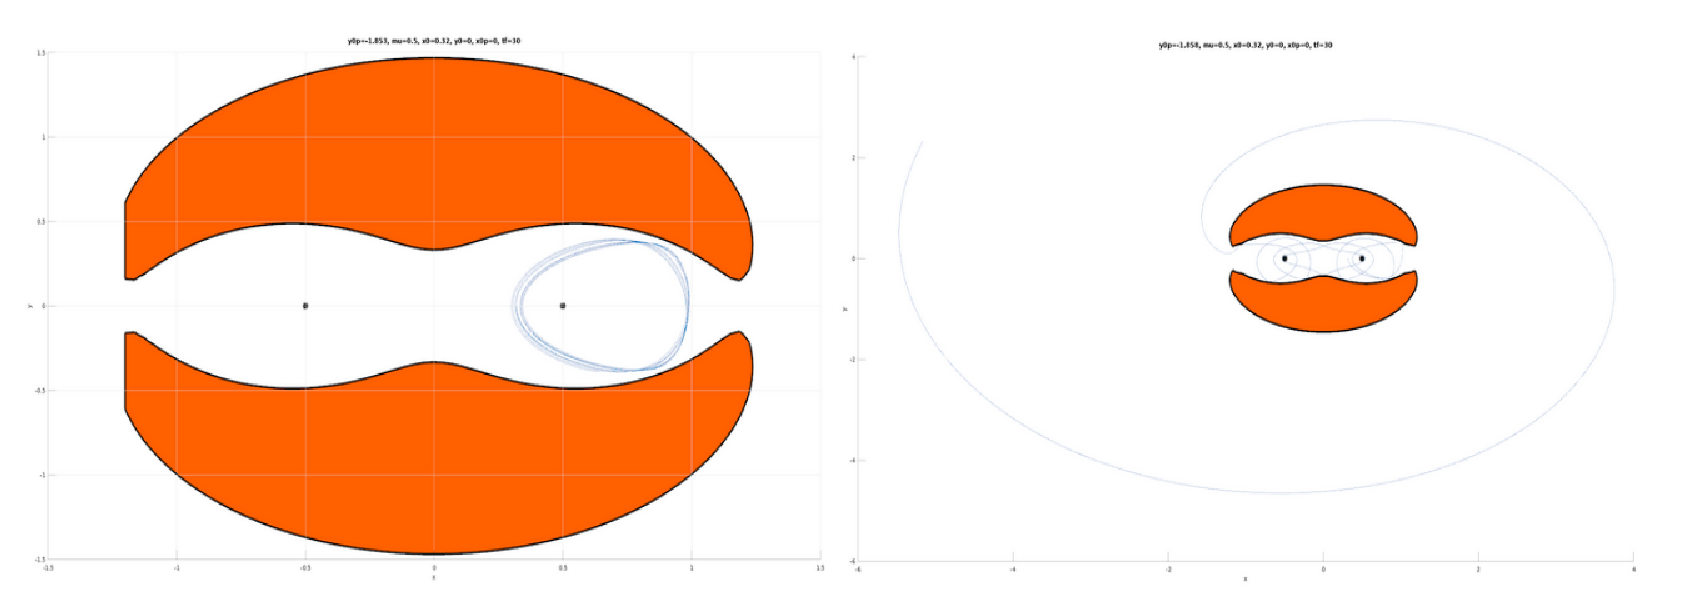
\includegraphics[width=16cm,height=5.5cm]{cont-third.eps}
\end{center}
\begin{center}
  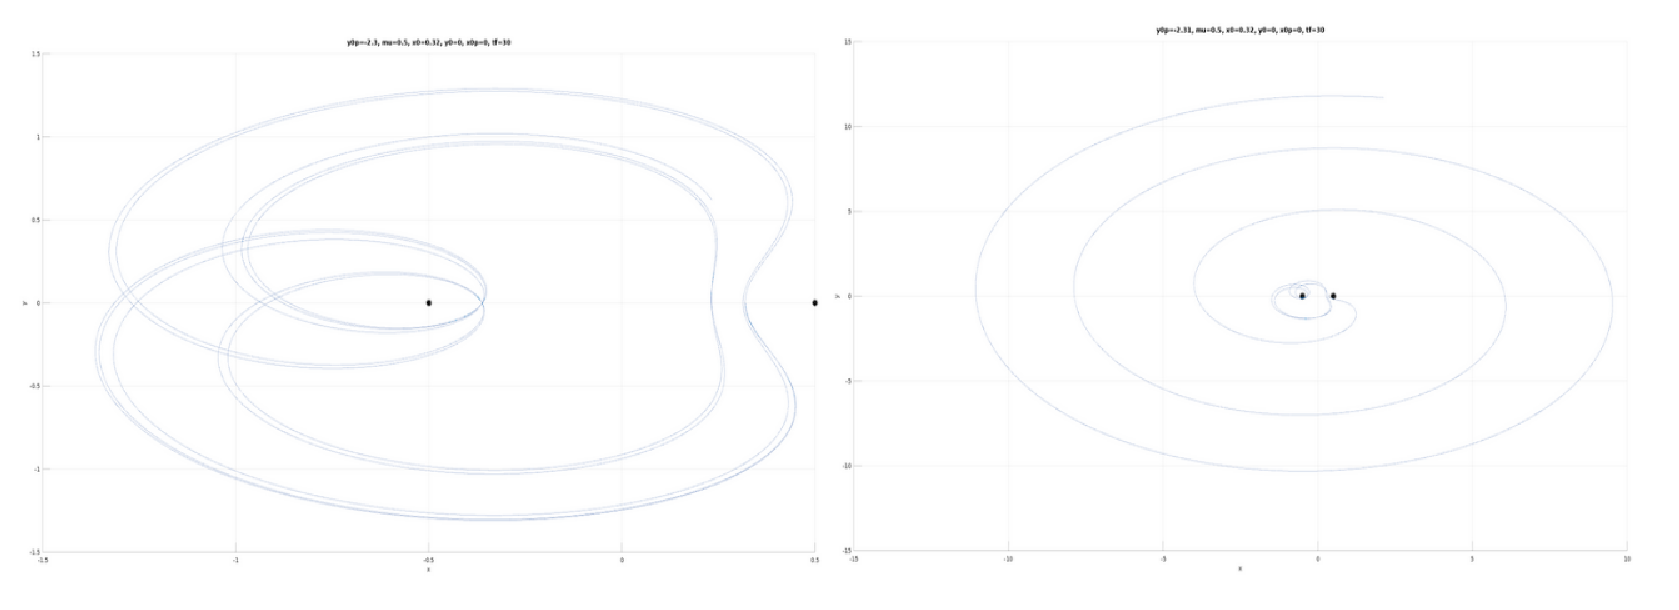
\includegraphics[width=16cm,height=5.5cm]{cont-fourth.eps}
\end{center}

\begin{center}
   \textit{Figure 9. Countour plots of the trajectories and the forbidden region. (upper left) Trajectory of a system with initial velocity parameter -1.853. (upper right) Trajectory of a system with initial velocity parameter -1.858. (lower left) Trajectory of a system with initial velocity parameter -2.3, and (lower right) shows the trajectory of a system with initial velocity parameter -2.31.}
\end{center}

Figure 9 shows that as the initial parameter for velocity keeps increasing, the forbidden region starts to increase until a point where it cannot be graphed in the selected boundaries. This forbidden region provides a useful guide to the size of the trajectory until a certain point, where the trajectory starts to move extremely far away from the two heavy bodies, mainly because of velocity and gravitational forces. 

Figure 9 also shows that as the velocity increases, the forbidden region loop starts to open, which means that the orbit of the smallest body can round any of the two heavy bodies at any given time based on its trajectories. When increasing the simulation times of the systems at higher velocities, trajectories tend to oscilate in longer cycles, which translates into longer trajectories around the two heavy bodies. It is important to note that as the velocity increases, Octave's Max step size option needs to be minimized to calculate trajectories appropiately and keep the selected maximum error tolerance.


\subsection{Possible Sources of Error}

Table 2 summarizes the solutions of the system when \textit{t} = 30. It is evident that as the initial velocity becomes more negative, the \textit{y} values also become more negative. Defining the ODE Absolute Tolerance and Max Step parameters produces more accurate results. The fact that in this problem the \textit{J} remains constant prevents any anomalies in the behavior of the solutions. In the initial velocities -2.3 and -2.31, the value for constant \textit{J} increases significantly (-0.79373 and -0.77068 respectively), when compared constant \textit{J’s} value at velocity -1.0 (-2.9387). The small difference between constant \textit{J} and the \textit{y} values may explain the issues while producing the contour plots at velocities -2.3 and -2.31.

\begin{table}[h!]
  \begin{center}
    \caption{Solutions of system (\ref{transform3}) when \textit{t} = 30.}
    \label{tab:table1}
    \begin{tabular}{c|c|c} 
      \textbf{$v_0$} & \textbf{x} & \textbf{y}\\
      \hline
      -1.000 & 0.38323 & -0.10938 \\
      -1.500 & 0.63632 & -0.11834 \\
      -1.730 & 0.58038 & -0.27020 \\
      -1.780 & 0.56670 & -0.29626 \\
      -1.853 & 0.54705 & -0.33162 \\
      -1.858 & 0.54573 & -0.33395 \\
      -2.300 & 0.44067 & -0.51058 \\
      -2.310 & 0.43856 & -0.51416 \\
      \hline
    \end{tabular}
  \end{center}
\end{table}

Many additional sources of numerical errors were present throughout this project. Starting with the least significant of the sources of error we have the floating-point decimal representation of the numbers in the computer. The computer that was used has a 64-bit CPU, thus the error is of order $O(10^{-16})$. Another apparent source of error is the $ode45$ function used to numerically solve these systems. By default, $ode45$ uses an adaptive timestep with an adaptive algorithm, but since it is a black-box ODE solver, we do not have specifics on the logical accuracy of the solver. This error was restricted by using the \textit{AbsTol} parameter, which tells the function to aim for an error that is smaller than the value of \textit{AbsTol}, and the \textit{MaxStep}, which forces the ODE solver to calculate the solutions at a lower time-step than its default. We used $AbsTol = 10^{-6}$ and $AbsTol = 10^{-3}$. Finally, by producing three-dimensional surf plots of the trajectories where the contour were not seen, we were able to discover that as the initial velocity increased, singularities will increase towards the negative side of the y-plane.

\begin{center}
  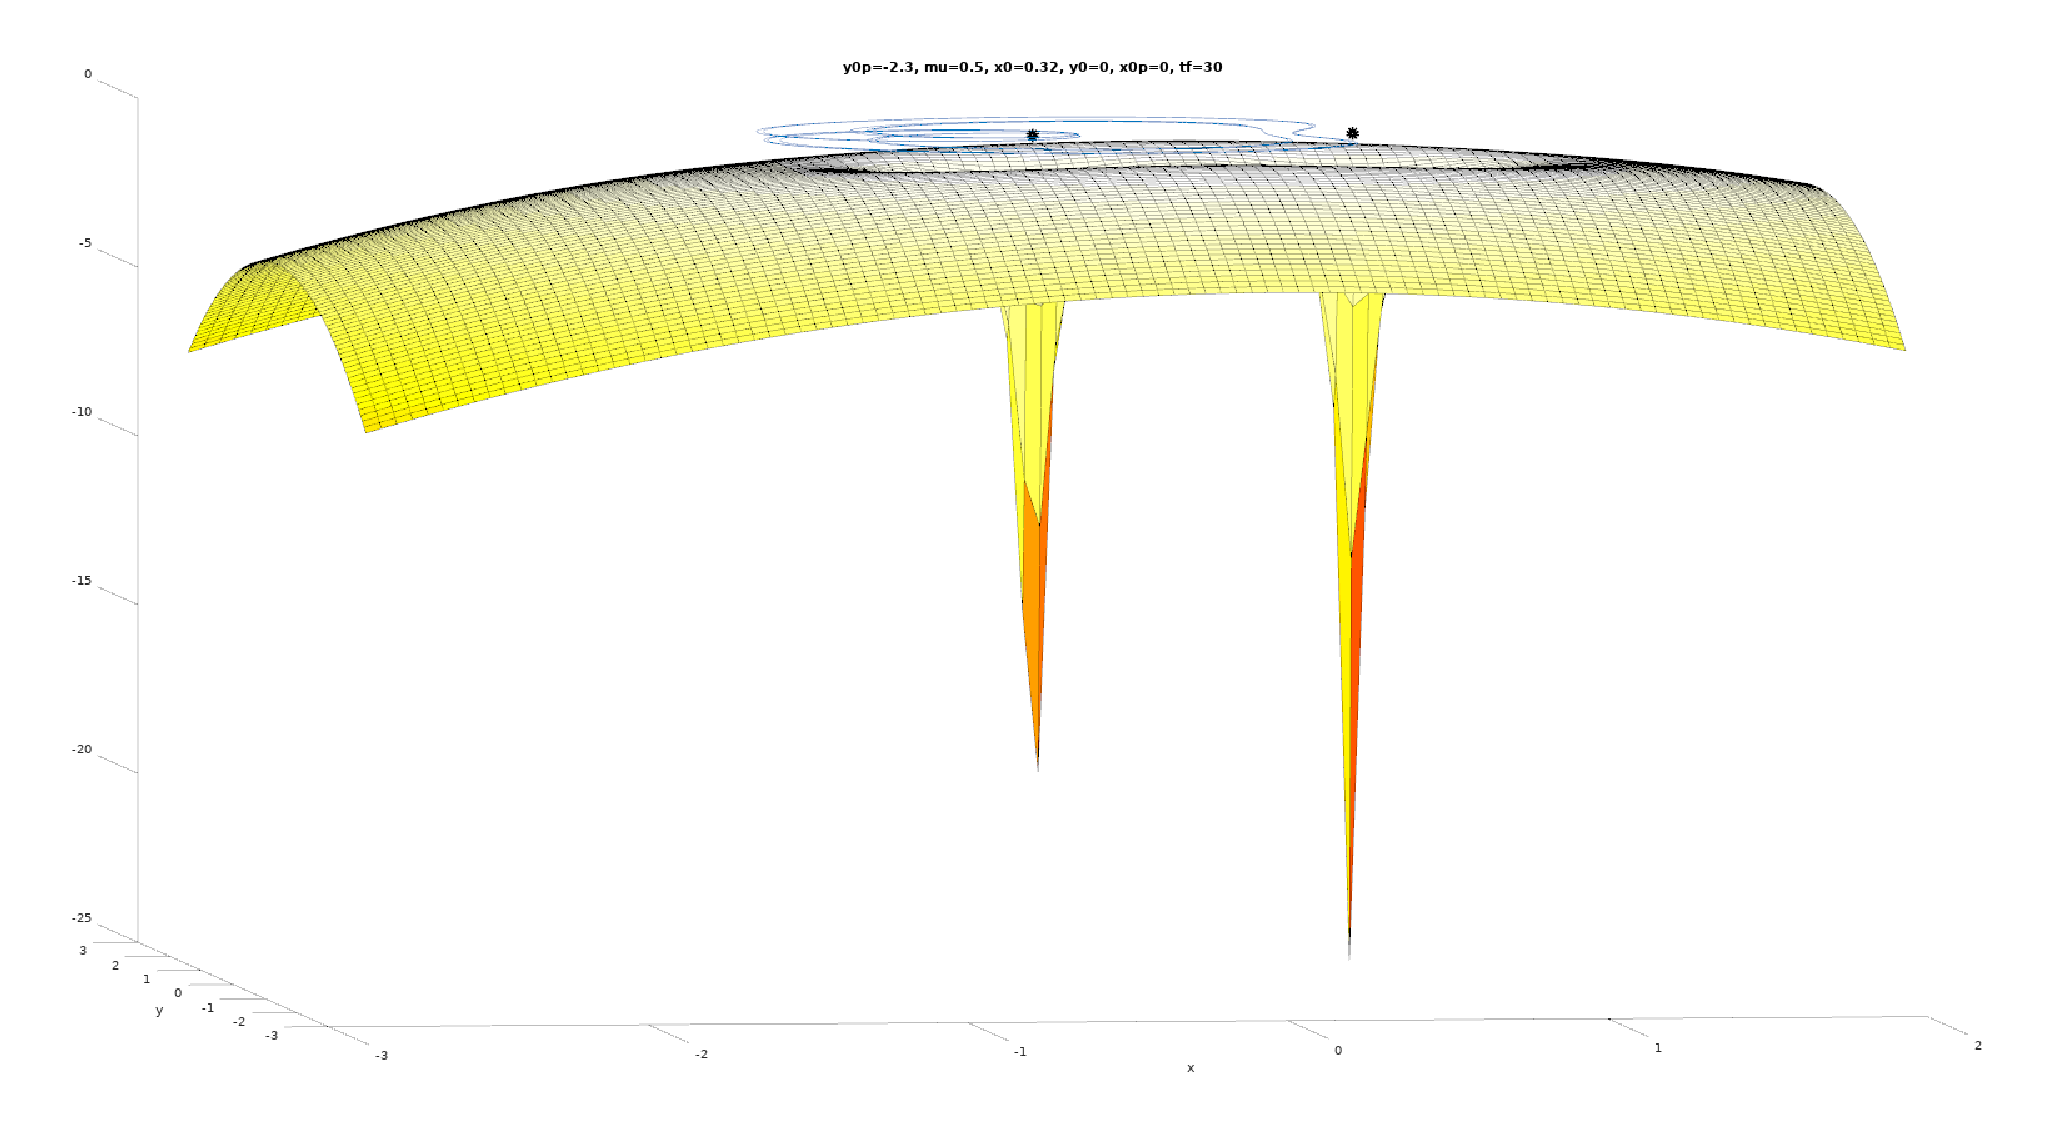
\includegraphics[width=14cm,height=5cm]{singularities.eps}
\end{center}

\begin{center}
  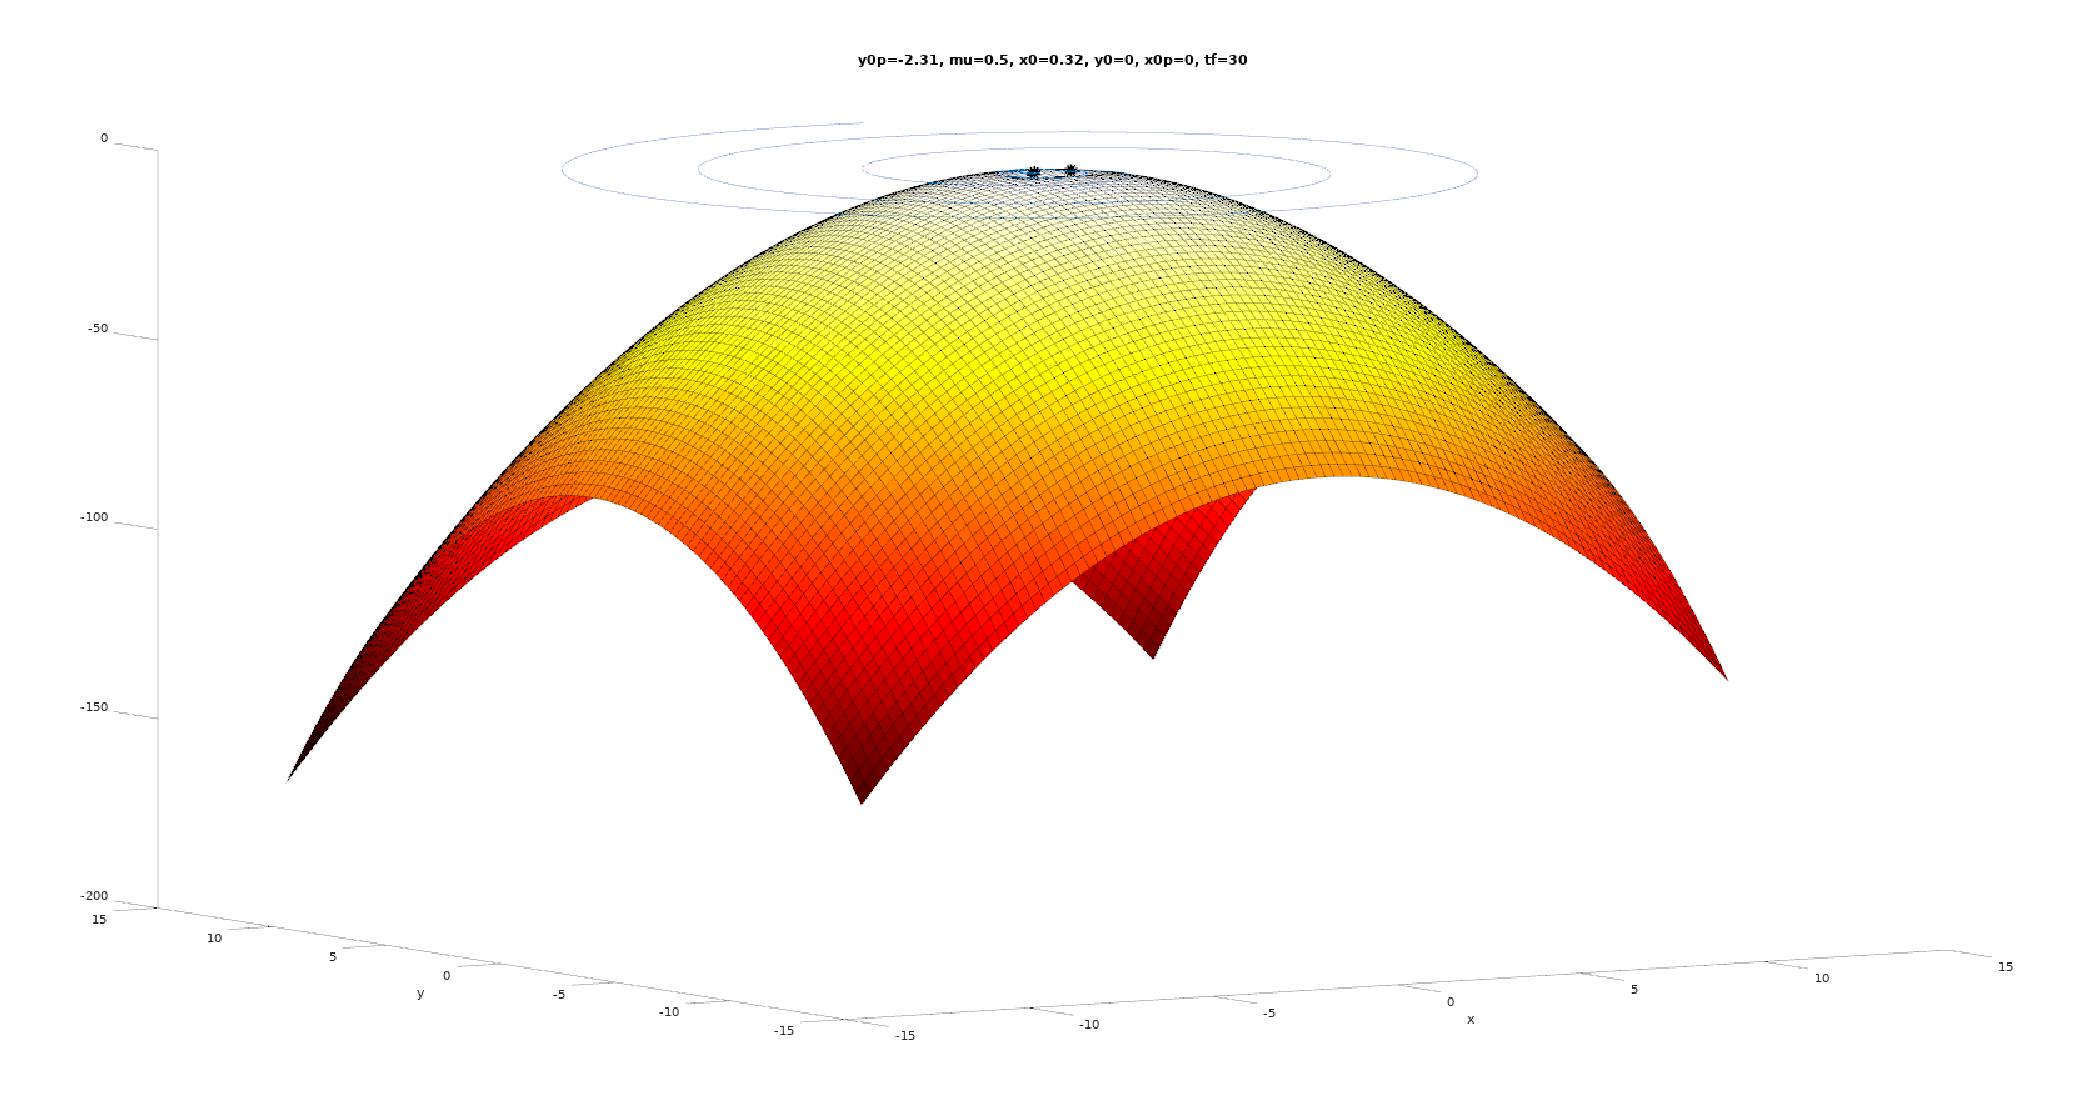
\includegraphics[width=14cm,height=5cm]{singularities231.eps}
\end{center}

\begin{center}
   \textit{Figure 10. Surf plot of the singularities regions from (upper) -2.3 and (lower) -2.31 velocities. Singularities start to move towards the negative y-plane as velocity increases.}
\end{center}


The singularities are the points where the smallest body would collide with one of the other larger bodies, so if we get too far from the singularities, the smallest body may escape the orbit of the two bigger bodies. One of the velocities used took the body into an orbit that spiraled outwards very fast, slowly escaping the gravitational influence the larger bodies had on it. Thus we can conclude that the singularities shown in Figure 10 represent the extreme increase in the trajectories of the system, which means that the trajectory of the smallest body escapes from the given boundaries of the plane.

\section{Conclusions}

The study of the three-body problem is of vital importance to the understanding of the interaction between spherical masses through gravitational forces described by Newton’s theory of gravity. In this manuscript we studied the restricted three-body problem by controlling specific initial parameters to simplify the proposed problem. Some of the cases studied were the general restricted three body problem with two of the heavy bodies being fixed to the x-plane, and the Copenhagen problem, where the small body is extremely close to one of the heavy bodies. This last problem lets us discard the centrifugal and gravitational forces from the furthest heavy body. A set of Octave programs were developed to simulate the orbit of the small body based on the conditions of the system and its forbidden region. Additional simulations were made to validate the effect of parameter changes in the system and to visualize these systems when increasing the simulation time. In conclussion, selected numerical methods were efficient to accurately calculate the trajectories of the proposed systems. Further improvements should be done to the proposed methods to enhance the speed and aspect of the given simulations.

\section{Future Work}

Future work includes additional simulations with higher initial parameters and simulation steps in order to analyze the impact in the trajectories given small and big variations. Since the three-body problem remains unsolved, further research should be conducted to find better numerical solutions to solve this problem. Finally, the theory discussed during this project should be applied to a given real situation during the Numerical Analysis class.

\section{Appendices}

This section includes a set of additional resources for the visualization of systems trajectories. Tutorials and supplementary code has been included. 

\subsection{Visualizing Continuous Trajectories}

A first Octave program was included in Section 2.4 to plot the trajectories of these systems based on given parameters. An adaptation to this program is included below to show the progress of the trajectories as they are being drawn. This program uses the hold on technique from Octave. Further improvements can be done to speed up this simulation.

\lstinputlisting[language=Octave]{simulation.m}

A video including one of the trajectories was generated and uploaded to YouTube (link=\href{https://www.youtube.com/watch?v=ne1JoJwG-Hc}{\textit{Simulation of the Restricted Three-Body Problem}}). Note that parameters are specified in the video description.

\subsection{Note to the Reader}

The following subsection was done to guide the reader on where to find the answers to the University of Cambridge lecture.

Question 1: Answered in section 2.4. Results discussed in section 3.1.

Question 2: Answered in section 2.5. Results discussed in section 3.2.

Question 3: Answered in section 2.6. Results discussed in sections 3.3 and 3.4.

% References

\newpage

\begin{thebibliography}{99}

\bibitem{Szebehely}{V. Szebehely, \textit{Theory of Orbits: The Restricted Problem of Three Bodies}, Academic Press Inc, 1967.}

\bibitem{Negron}{P. Negr\'{o}n, \textit{Ecuaciones Diferenciales Ordinarias}, UPR-Humacao, 2017.}

\bibitem{Musielak}{Z. E. Musielak, B. Quarles, \textit{The three-body problem}, Reports on Progress in Physics, 2014.}

\bibitem{Frank}{J. Frank, \textit{The Three-Body Problem}, Special Lecture LSU, 2006.}

\bibitem{Marchal}{M. Christian. \textit{The three-body problem}. Elsevier, 2012.}

\bibitem{Philip}{B., Philip G., et al. \textit{Newton vs the machine: solving the chaotic three-body problem using deep neural networks.} arXiv preprint arXiv:1910.07291 (2019).}

\end{thebibliography}

\end{document}


